\documentclass[12pt]{article}
\usepackage[margin=2.5cm]{geometry}
\usepackage{enumerate}
\usepackage{amsfonts}
\usepackage{amsmath}
\usepackage{fancyhdr}
\usepackage{amsmath}
\usepackage{amssymb}
\usepackage{amsthm}
\usepackage{mdframed}
\usepackage{graphicx}
\usepackage{subcaption}
\usepackage{listings}
\usepackage{xcolor}
\usepackage{booktabs}
\usepackage[utf]{kotex}

\definecolor{codegreen}{rgb}{0,0.6,0}
\definecolor{codegray}{rgb}{0.5,0.5,0.5}
\definecolor{codepurple}{rgb}{0.58,0,0.82}
\definecolor{backcolour}{rgb}{0.95,0.95,0.92}

\lstdefinestyle{mystyle}{
    backgroundcolor=\color{backcolour},
    commentstyle=\color{codegreen},
    keywordstyle=\color{magenta},
    numberstyle=\tiny\color{codegray},
    stringstyle=\color{codepurple},
    basicstyle=\ttfamily\footnotesize,
    breakatwhitespace=false,
    breaklines=true,
    captionpos=b,
    keepspaces=true,
    numbers=left,
    numbersep=5pt,
    showspaces=false,
    showstringspaces=false,
    showtabs=false,
    tabsize=1
}

\lstset{style=mystyle}

\begin{document}
\title{CSC148 Worksheet 9 Solution}
\author{Hyungmo Gu}
\maketitle

\section*{Question 1}
\begin{figure}[h!]
    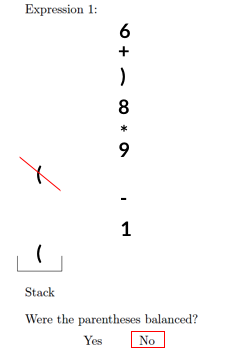
\includegraphics[width=0.45\textwidth]{images/worksheet_9_q1a_solution.png}\hfill
    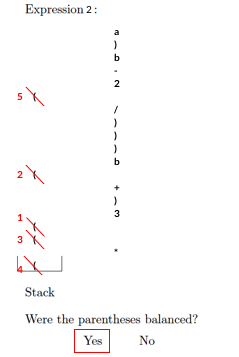
\includegraphics[width=0.45\textwidth]{images/worksheet_9_q1b_solution.png}\hfill
\end{figure}

\begin{figure}[h!]
    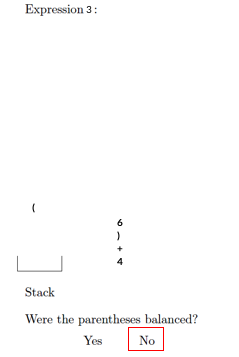
\includegraphics[width=0.45\textwidth]{images/worksheet_9_q1c_solution.png}\hfill
\end{figure}

\newpage

\section*{Question 2}
\begin{enumerate}[a.]
    \item

    For each character being received,

    \begin{enumerate}[1.]
        \item If the character is left parenthesis, then we need to store it in stack using \textit{push()} method
        \item If the character is right parenthesis
        \begin{enumerate}[1.]
            \item First, check for the non-emptiness of stack.
            \item If the list is not empty, then we need to pop an element form stack.
            \item If list is empty, then we need to raise error.
        \end{enumerate}
        \item If the character is other than left or right parenthesis, then pass the character.
    \end{enumerate}

    \item We will know the parenthesis are balanced when the number of elements
    in stack is zero after traversing a string.
\end{enumerate}

\section*{Question 3}
\begin{lstlisting}[language=Python,caption={worksheet\_9\_q3\_solution.py},captionpos=b]
    def is_balanced(line: str) -> bool:
        """Return whether <line> contains balanced parentheses.

        Ignore square and curly brackets.

        >>> is_balanced('(a * (3 + b))')
        True
        >>> is_balanced('(a * (3 + b]]') # Note that the two ']'s don't matter
        False
        >>> is_balanced('1 + 2(x-y)}') # Note that the '}' doesn't matter
        True
        >>> is_balanced('3 - (x')
        False
        """
        parenthesis_stack = Stack()

        for character in line:
            # If the character is left parenthesis,
            if character == '(':
                # Store it in stack
                parenthesis_stack.push('(')
            # If the character is right parenthesis,
            elif character == ')':
                # Check for the non-emptiness of stack.
                if parenthesis_stack.is_empty():
                    # if empty, return false.
                    return False

                # If the list is not empty, then pop an element form stack.
                parenthesis_stack.pop()

        # Check parenthesis are balanced by checking stack is empty.
        if not parenthesis_stack.is_empty():
            return False

        return True
\end{lstlisting}

\section*{Question 4}
\begin{lstlisting}[language=Python,caption={worksheet\_9\_q4\_solution.py},captionpos=b]
    def is_balanced(line: str) -> bool:
        """Return whether <line> contains balanced parentheses.

        >>> is_balanced('abc')
        True
        >>> is_balanced('(a * (3 + b))')
        True
        >>> is_balanced('(a * (3 + b]]')
        False
        >>> is_balanced('(a * [3 + b])')
        True
        >>> is_balanced('1 + 2(x-y)}')
        False
        >>> is_balanced('{3 + [2 * 4(x-y)]}')
        True
        >>> is_balanced('3 - (x')
        False
        """
        brackets_stack = Stack()

        for character in line:
            # If the character is one of '[', '{'. or '(',
            if (character == '(' or
                character == '[' or
                character == '{'):
                # Store it in stack
                brackets_stack.push(character)
            # If the character is one of ']', '}', or ')',
            elif (character == ')' or
                character == ']' or
                character == '}'):
                # Check for the non-emptiness of stack.
                if brackets_stack.is_empty():
                    # if empty, return false.
                    return False

                # If the list is not empty, then pop an element form stack.
                left_bracket = brackets_stack.pop()

                # If popped bracket doesn't match, then return false
                if ((left_bracket == '(' and character != ')') or
                    (left_bracket == '[' and character != ']') or
                    (left_bracket == '{' and character != '}')):

                    return False


        # Check parenthesis are balanced by checking stack is empty.
        if not brackets_stack.is_empty():
            return False

        return True
\end{lstlisting}


\end{document}